\begin{figure}
  \centering
  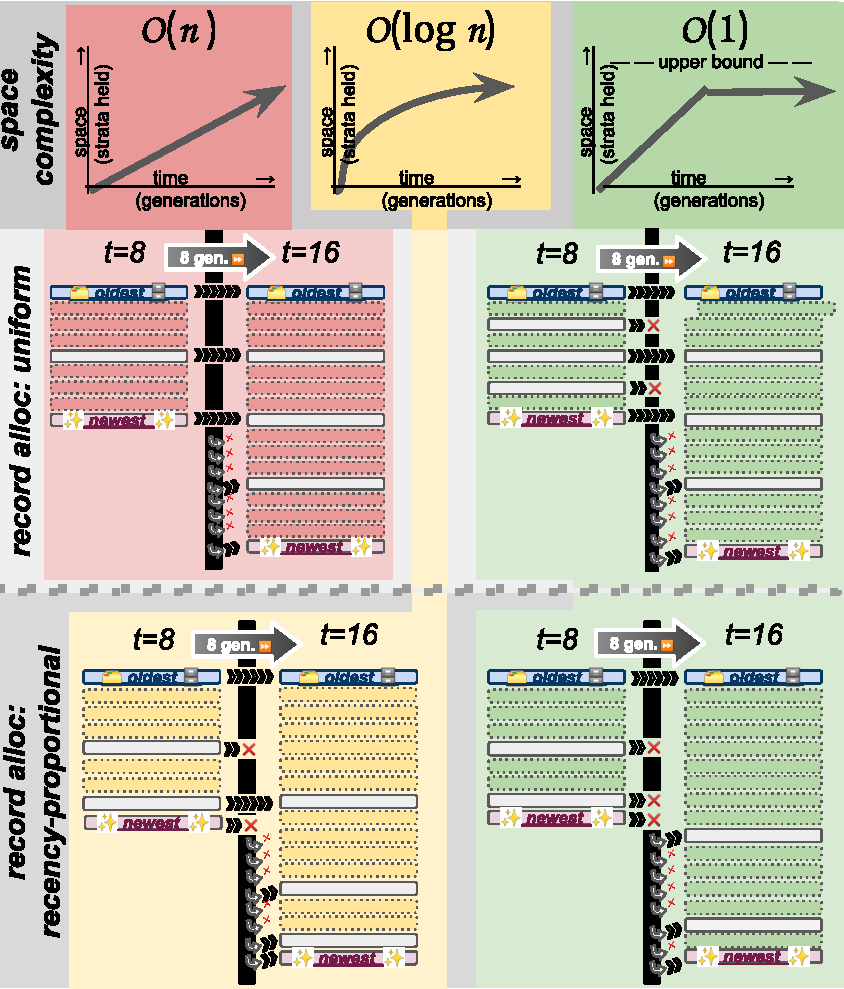
\includegraphics[width=\textwidth]{img/retention-policy-matrix}
  \caption{
    Comparison of four stratum retention policies by space complexity per stratigraph with respect to generations elapsed (columns, red/yellow/green) and by distribution of retained differentia (rows).
    Uniform allocation keeps differentia in evenly-spaced layers.
    Recency-proportional allocation keeps more more-recent differentia, trading off coarser resolution to infer ancient phylogenetic events for finer resolution to infer recent phylogenetic events.
    Retained layers under each policy are shown at $t=8$ generations and $t=16$ generations, with new differentia being deposited in a descending fashion.
    Differentia pruning events are noted with a red $x$.
  }
  \label{fig:retention-policy-matrix}
\end{figure}
